% XCircuit output "cto_ej2_1ciclo.tex" for LaTeX input from cto_ej2_1ciclo.eps
\def\putbox#1#2#3#4{\makebox[0in][l]{\makebox[#1][l]{}\raisebox{\baselineskip}[0in][0in]{\raisebox{#2}[0in][0in]{\scalebox{#3}{#4}}}}}
\def\rightbox#1{\makebox[0in][r]{#1}}
\def\centbox#1{\makebox[0in]{#1}}
\def\topbox#1{\raisebox{-0.60\baselineskip}[0in][0in]{#1}}
\def\midbox#1{\raisebox{-0.20\baselineskip}[0in][0in]{#1}}
   \scalebox{1}{
   \normalsize
   \parbox{4.00521in}{
   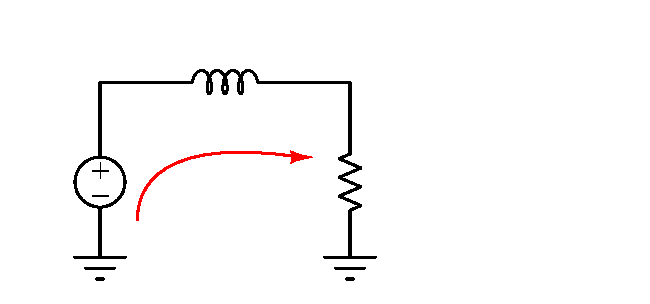
\includegraphics[scale=1]{cto_ej2_1ciclo}\\
   % translate x=1024 y=60 scale 0.38
   \putbox{1.22in}{1.62in}{1.20}{L1}%
   \putbox{1.22in}{1.04in}{1.20}{20u}%
   \putbox{2.39in}{0.79in}{1.20}{$RDS<on>$}%
   \putbox{2.39in}{0.54in}{1.20}{$0,0375 \Omega$}%
   \putbox{0.06in}{0.70in}{1.20}{V1}%
   \putbox{0.06in}{0.45in}{1.20}{12V}%
   \putbox{1.14in}{0.62in}{1.20}{\textcolor{red}{IL1}}%
   } % close 'parbox'
   } % close 'scalebox'
   \vspace{-\baselineskip} % this is not necessary, but looks better
